\documentclass[11pt,a4paper,openright]{memoir}
% \usepackage[utf8]{inputenc}
\usepackage{csquotes}
\usepackage{graphicx}
\usepackage{url}
\usepackage{soul}
\usepackage{multicol}
\usepackage[document]{ragged2e}
\usepackage[backend=bibtex,bibencoding=ascii]{biblatex}
\addbibresource{thesis.bib} 

\usepackage{unswcover} % This one includes babel in Australian mode

\newcommand{\theTitle}{Knowledge graph construction for research literatures}
\newcommand{\theAuthor}{Alisson Oldoni}
\newcommand{\theKeywords}{natural language processing, information extraction, name entity recognition, relationship extraction}

\unswschool{School of Computer Science and Engineering\\}
%% PhD is the default
\unswdegree{Master of Computing and Information Technology}
%\unswcotutelle{Dép. Mathématiques et Systèmes---Centre de Robotique\\
% École Nationale Supérieure des Mines--ParisTech, France}
%% Needed for final submission
%\unswdissertationsheet{unsw_thesis_dissertation_sheet.pdf}

\usepackage[unicode]{hyperref}
\hypersetup{colorlinks=true, linkcolor=black, citecolor=black, urlcolor=blue,
  pdftitle={\theTitle}, pdfauthor={\theAuthor}, pdfkeywords={\theKeywords}}

\title{\theTitle}
\author{\theAuthor}
\newsavebox{\compiledate}
\savebox{\compiledate}{\begin{otherlanguage}{australian}\today\end{otherlanguage}}
%\date{\today (document compilation)}
%% By forcing the date as follows, we let Babel do its job of formatting it
%% properly
\renewcommand\day{14}
\renewcommand\month{12}
\renewcommand\year{2011}

\begin{document}
\setlength\parindent{24pt}
\captionnamefont{\bfseries}

\frontmatter

%% If only the title page is desired
%\makeunswphdtitlepage
%% If all the administrative pages are needed too
\makeunswfrontmatter

\newpage
\thispagestyle{empty}
\strut
\vfill

%\chapter*{Acknowledgements}
%\pdfbookmark{Acknowledgements}{pdfmark:ack}
%Thanks to Camila Macagnan, my wife, for supporting through this whole process.
%I would like to thank my professor Dr. Wei Wang for all the help into delivering this project.

\chapter*{Abstract}
\pdfbookmark{Abstract}{pdfmark:abs}

%\cleardoublepage
\clearpage
\tableofcontents

\cleardoublepage
%\listoffigures

\mainmatter

\chapter{Introduction}
A Knowledge Graph (KG), also known as the knowledge base, is a collection of the machine-readable database that contains entities, the attributes of entities and the relationships between entities \cite{google}. It is an essential foundation for many applications that requires machine understanding.

Popular search engines such as Google \cite{google} and Bing \cite{bing} are all leveraging Knowledge Graphs as to provide entity summary information and the related entities based on the query that the user is searching for.

\begin{figure}[!htbp]
  \centering
    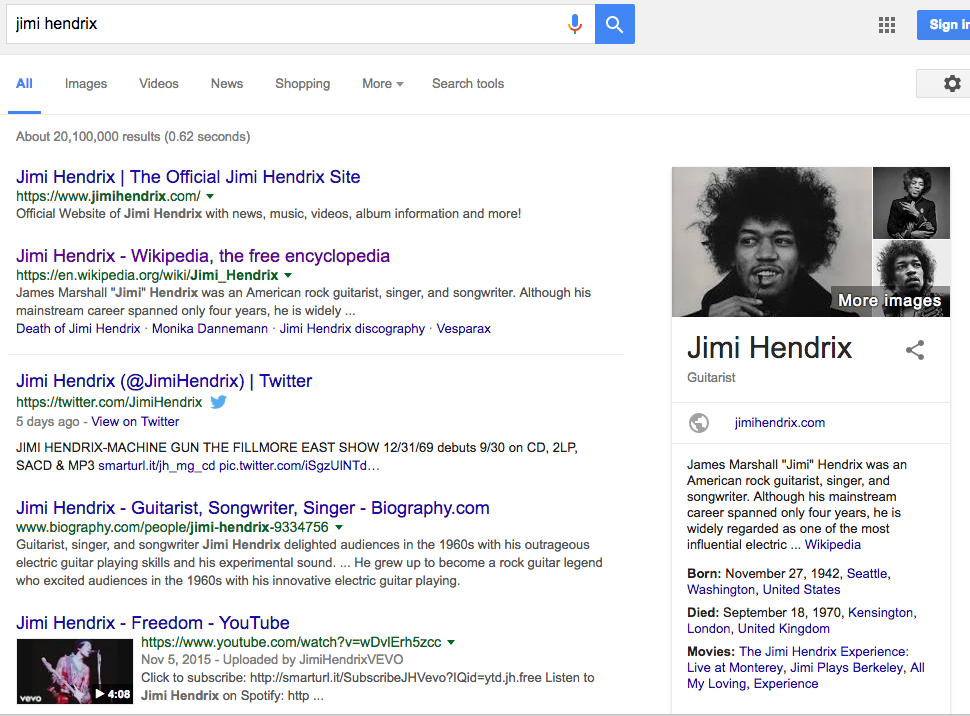
\includegraphics[width=0.8\textwidth]{./images/google_knowledge_graph}
  \caption[An example of knowledge graph application.]{An example of knowledge graph application in the Google's result page.}
  \label{fig:google_knowledge_graph}
\end{figure}

The use of Knowledge Graphs then allow users to be able to see extra information in a summarised table-like form, as to resolve their query without having to navigate to other sites. Note in the example in Figure \ref{fig:google_knowledge_graph} how the right column represents a sequence of facts of the \emph{Jimi Hendrix} entity, in this case an entity of the class (or type) \emph{person}, such as: his official website; where and when he was born; where and when he died; and a list of movies where this person is the subject of.

In this project, we focus on building a domain-specific knowledge graph from research literatures. More specifically, we focus on papers from the topic of databases and attempt to extract information from these papers in order to build a knowledge graph. The first step to achieve in achieving our goal is obtaining the raw natural language text from papers n the area. Most research products such as thesis, papers, or any other report, are mostly available primarily in the Portable Document Format (PDF) format \cite{pdf} - which then needs to then be parsed into a raw text in an automated manner. Once this text is available, it is then parsed and processed into the following workflow:
\begin{enumerate}
  \item Discover entities in the text;
  \item Discover relationships between these entities;
  \item Design effective and efficient algorithms to extract entities and relationships;
  \item \hl{Perform entity disambiguation and linking to a reference Knowledge Graph (e.g., Yago2 or DBPedia).}
  \item Improve the quality of the output via input data cleaning, robust extraction, and learning-based post-processing methods;
  \item Presenting the facts in a graph (the Knowledge Graph).
\end{enumerate}

In the next sections, this document will give some background information on the techniques needed to achieve the above (Chapter 2), and it will also define the problem more precisely (Chapter 3), building as to introduce the development of this research (Chapter 4). In Chapter 5 we will describe some of the results, followed by the some final remarks in Chapter 6.


\chapter{Information Extraction from Natural Language Text}

In this project, we focus on building a domain-specific knowledge graph for research literatures. A similar service is the Semantic Scholar \cite{semanticscholar} project by Professor Oren Etzioni from Allen Institute for AI. However, Semantic Scholar can only understand a very limited number of relationships (such as 'cite', 'comment', 'use\_data\_set', and 'has\_caption'), \hl{and it does not offer entity disambiguation (e.g., mixing all "Wei Wang"'s publication together)}.

\section{Knowledge Graphs}

Knowledge Graphs contain a valuable of information in a structured format, traditionally originally mined from table-like structures form places like Wikipedia \cite{wiki} tables \cite{dbpedia-swj}. It can be used for a diverse range of applications, such as helping other systems reason about quality of harvested facts\cite{Suchanek2007}, provide table-like facts about an entity\cite{google}, and question-answering systems\cite{hixon-clark-hajishirzi-2015}. Moreover, recent years have witnessed a surge in large scale knowledge graphs, such as DBpedia \cite{dbpedia-swj}, Freebase \cite{Bollacker2008}, Google’s Knowledge Graph \cite{google}, and YAGO \cite{Suchanek2007}.

The Knowledge Graph name follows from the data structure that is created from the facts in its final form, a graph with nodes representing entities and edges representing various relations between entities. In Figure \ref{fig:yago_knowledge_graph}, it is possible to observe an example plotted in this form. The list of possible entities classes, and allowable relations between entities is known as a schema. The schema represented in Figure \ref{fig:yago_knowledge_graph} is detailed in Table \ref{tab:max_planck}; one can observe that, as an example, \emph{Max Planck} is an entity of the type \emph{physicist}.

\begin{table}[!htbp]
  \centering
  \RaggedRight
    \texttt{type(A, D) :- type(A, B), subclassOf(B, C), subclassOf(C, D)} \\
  \caption[An example of entailment.]{This entailment example allows one to assert that \texttt{type(Max Planck, person)} is also true, based on the fact tuples presented in Table \ref{tab:max_planck}.}
  \label{tab:entailment_example_max}
\end{table}

Moreover, based on the facts presented, entailments can be made and one trivial example is denoted in Table \ref{tab:entailment_example_max}. More complex examples of possible reasoning can be seen in \cite{Surdeanu:2011:CIE:2021153.2021155}. This is equivalent to traversing the graph from a node that represents a more specific information, to a node that represents a more general information - e.g.: another possible child node of \emph{scientist} could be the type \emph{biologist}.

\begin{table}[!htbp]
  \centering
  \RaggedRight
    \texttt{type(Max Planck, physicist)} \\
    \texttt{subclassOf(physicist, scientist)} \\
    \texttt{subclassOf(scientist, person)} \\
    \texttt{bornIn(Max Planck, Kiel, 1858)} \\
    \texttt{type(Kiel, city)} \\
    \texttt{locatedIn(Kiel, Germany)} \\
    \texttt{hasWon(Max Planck, Nobel Prize, 1919)} \\
  \caption[Some facts regarding Max Planck.]{Some facts regarding Max Planck, also depicted in Figure \ref{fig:yago_knowledge_graph}.}
  \label{tab:max_planck}
\end{table}

This example denotes a classical domain, more precisely important persons, companies, locations, and the relations between them, in which Information Extraction (IE) tools have been very successful on.

\begin{figure}[!htbp]
  \centering
    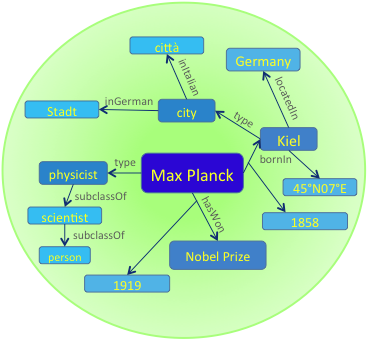
\includegraphics[width=0.6\textwidth]{./images/yago_graph}
  \caption[An example of knowledge graph plotted with vertices and edges.]{An example of knowledge graph from \cite{Suchanek2007} plotted with vertices and edges.}
  \label{fig:yago_knowledge_graph}
\end{figure}

As mentioned previously, YAGO \cite{Suchanek2007} is a prominent Knowledge Graph database, and possesses several advanced characteristics. Every relation in its database is annotated with its confidence value. See the example of the resulting graph in Figure \ref{fig:yago_examples}. Moreover, YAGO combines the provided taxonomy with WordNet \cite{Miller:1995:WLD:219717.219748} and with the Wikipedia category system \cite{wiki}, assigning the entities to more than 350,000 classes. This allow for very powerful querying. Finally, it attaches a temporal and a spacial dimension to many of its facts and entities, being then capable to answer questions such as \emph{when} and \emph{where} such event took place.

WordNet is a semantically-oriented dictionary of English, similar to a traditional thesaurus but with a richer structure \cite{BirdKleinLoper09}. More specifically, it provides relations to synonyms, hypernyms and hyponyms, among others.

\begin{figure}[!htbp]
  \centering
    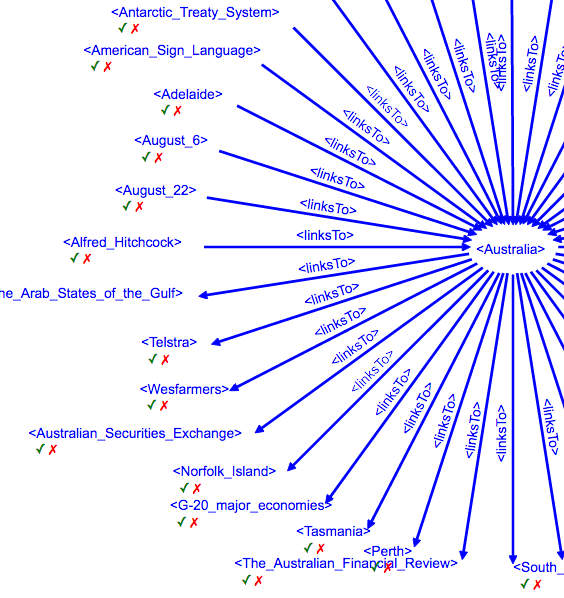
\includegraphics[width=0.6\textwidth]{./images/yago}
  \caption[An example of patterns existants in YAGO.]{An example of patterns existants in YAGO.}
  \label{fig:yago_examples}
\end{figure}

\section{Information Extraction}

Information extraction (IE) is the process of obtaining in an automatic fashion facts and information from unstructured text that can be read by a machine \cite{Jurafsky:2000:SLP:555733}. Also according to \cite{Jurafsky:2000:SLP:555733}, the IE process is, in general, divided in the following subtasks: Named Entity Recognition (NER), Coreference Resolution, Entity Disambiguation, Relation Extraction (RE), Event Detection, Temporal Analysis. The main subtasks relevant to this report will be described further in this section.

Once the information is extracted it is then used for tasks such as Template Filling \cite{Jurafsky:2000:SLP:555733}, or stored as a Knowledge Graph for downstream logical reasoning or for further queries.

\begin{table}[!htbp]
  \centering
  \RaggedRight
    [\textsubscript{PER} James Cook] was born on 27 October 1728 in the village of [\textsubscript{LOC} Marton] in [\textsubscript{COUNTY} Yorkshire].
  \caption[An example of NER.]{An example of Named Entity Recognition (NER).}
  \label{tab:james_cook}
\end{table}

Name Entity Recognition is the process of, given a sentence, mark what are the entities that are part of it. Once the entity is detected, it needs to be classified within the classes of the given domain - in the spirit of the previous examples this would be e.g.: \emph{City} or \emph{Person}. A few approaches exist for the problem of NER, mostly related to Pattern Matching or Sequence Classification.

\begin{table}[!htbp]
  \centering
    \begin{tabular}{ll}
      \textbf{Pattern}          & \textbf{Would yield ENTITY of type} \\
      {[PERSON]} was born       & PERSON            \\
      in the village of {[LOC]} & LOCATION          \\
      in {[LOC]}                & LOCATION           
    \end{tabular}
  \caption[Patterns for NER.]{Examples of Named Entity Recognition (NER) patterns, based on the sentence from Table \ref{tab:james_cook}.}
  \label{tab:james_cook_patterns}
\end{table}

Observe, for an example, the sentence in Table \ref{tab:james_cook}. Several articles regarding prominent figures, either historical or of our current society, can start with the text \emph{[ENTITY] was born}. One approach might be Pattern Matching, which is to mine the input natural language text while looking for this pattern using Regular Expressions - or a Finite-State Automata \cite{Jurafsky:2000:SLP:555733}. The entities found by this pattern would then also receive the \emph{person} class. Other possible patterns can be found in Table \ref{tab:james_cook_patterns}.

Another way to extract entities from text is to frame the NER problem as a Sequence Classification problem. It requires the training of a classifier in which, given the class of the previous word, and other surrounding features of the current word, will attempt to guess if the current word is an entity, and if it is, also guesses its class.

To achieve this, previously annotated data with existing sentences and its entities is needed. The format in which this annotated data is provided varies, however more commonly the IOB format (Table \ref{tab:james_cook_iob}) is used in several of the NER tools, including NLTK \cite{BirdKleinLoper09} and the popular Stanford Named Entity Recognizer (NER), part of the Stanford CoreNLP \cite{manning-EtAl:2014:P14-5}. Stanford CoreNLP provides a set of natural language analysis tools.

\begin{table}[!htbp]
  \centering
    \begin{tabular}{ll}
      \textbf{Word}          & \textbf{Tag} \\
      James                  & B-PERSON \\
      Cook                   & I-PERSON \\
      was                    & O \\
      born                   & O \\
      on                     & O \\
      27                     & B-DATE \\
      October                & I-DATE \\
      1728                   & I-DATE \\
      in                     & O \\
      the                    & O \\
      village                & O \\
      of                     & O \\
      Marton                 & B-LOC \\
      in                     & O \\
      Yorkshire              & B-LOC \\
      .                      & O \\
    \end{tabular}
  \caption[IOB-formatted sentence.]{Example of IOB-formatted sentence used to train classifiers for the Named Entity Recognition (NER) task, based on the sentence from Table \ref{tab:james_cook}.}
  \label{tab:james_cook_iob}
\end{table}

The IOB format also helps remove ambiguity in case there are two contiguous entities of same class without any word tagged as \emph{O} in between. In practice, these cases are somewhat rare in several domains, and thus a simplified version without the \emph{B-} and \emph{I-} prefixes are used \cite{Surdeanu:2011:CIE:2021153.2021155}.

The Stanford Named Entity Recognizer (NER), also known as CRFClassifier \cite{Finkel:2005:INI:1219840.1219885}, provides a general implementation of (arbitrary order) linear chain Conditional Random Field (CRF) sequence models. A CRF is a conditional sequence model which represents the probability of a hidden state sequence given some observations.

Several useful features can be used during the training of a NER CRF classifier model. In Table \ref{tab:ner_features}, several examples are presented. The Word Shape feature is an interesting addition from recent research, as it captures the notion that most entities are written in capital letters, or starting with capital letter, or containing numbers in the middle of the word, and other specific shapes.

\begin{table}[!htbp]
  \centering
    \begin{tabular}{ll}
      \textbf{Feature}          & \textbf{Description} \\
      Word                      & The current word being classified.          \\
      N-grams                   & \parbox[t]{9cm}{A feature from n-grams, i.e., sub-strings of the word.} \\
      Previous Class            & The class of the immediate previous word.          \\
      Previous Word             & The previous word.          \\
      Disjunctive               & \parbox[t]{9cm}{Disjunctions of words anywhere in the left or right.} \\
      Word Shape                & \parbox[t]{9cm}{The shape of the word being processed captured using. In general replaces numbers with \emph{d}, \emph{x} to lower-case letters, and \emph{X} to upper-case letters.} \\
    \end{tabular}
  \caption[Possible features to train the CRFClassifier.]{Examples of features used to train the CRFClassifier.}
  \label{tab:ner_features}
\end{table}

In addition to the above methods another useful technique is the use of gazetteers. Gazetteers are common for geographical data, where government provided lists of names can contain millions of entries names for all manner of locations along with detailed geographical, geologic and political information \cite{Jurafsky:2000:SLP:555733}.

Relation Extraction (RE) is the ability to discern the relationships that exist among the entities detected in a text \cite{Jurafsky:2000:SLP:555733}, and is naturally the next challenge after being able to detect entities. It can be done using Pattern Matching, Classifiers, or purely by exploiting linguistic data available form a sentence.

The Pattern Matching technique from NER is then built upon in the Relation Extraction step, and now involves more than one entity, yielding binary relations. This approach is used in tools such as PROSPERA \cite{Nakashole:2011:SKH:1935826.1935869} or those mined by PATTY \cite{Nakashole:2012:PTR:2390948.2391076}. More specifically, examples of patterns mined by PATTY for the \emph{graduatedFrom} relation are seen in Figure \ref{fig:patty_examples}.

\begin{figure}[!htbp]
  \centering
    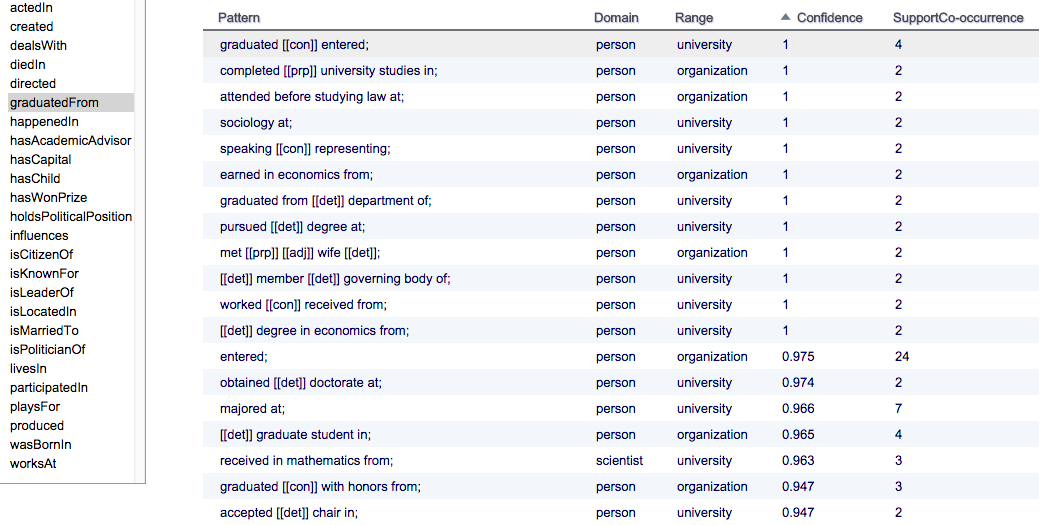
\includegraphics[width=0.8\textwidth]{./images/patty}
  \caption[An example of patterns extracted from PATTY.]{An example of patterns extracted from PATTY for the \emph{graduatedFrom} relation.}
  \label{fig:patty_examples}
\end{figure}

PROSPERA's main technique is that not only it obtain facts based on a small set of initial seed patterns, but also obtain new candidate patterns based on the mined facts. Once the process finishes, these new candidate patterns are evaluated and then added to the the existing pattern repository for re-use. The whole process then iterates again finding even more facts from these new patterns, and new candidate patterns.

Another tool in the Stanford CoreNLP package, the Relation Extractor \cite{Surdeanu:2011:CIE:2021153.2021155} is a classifier to predict relations in sentences.

The RMD model was built from scratch as a multi-class classifier that extracts binary relations between entity mentions in the same sentence. Dur- ing training, known relation mentions become pos- itive examples for the corresponding label and all other possible combinations between entity men- tions in the same sentence become negative exam- ples. We used a multiclass logistic regression classi- fier with L2 regularization. Our feature set is taken from (Yao et al., 2010; Mintz et al., 2009; Roth and Yih, 2007; Surdeanu and Ciaramita, 2007) and mod- els the relation arguments, the surface distance be- tween the relation arguments, and the syntactic path between the two arguments, using both constituency and dependency representations. For syntactic in- formation, we used the Stanford parser (Klein and Manning, 2003) and the Stanford dependency repre- sentation (de Marneffe et al., 2006).
For RMD, we implemented an additive feature se- lection algorithm similar to the one in (Surdeanu et al., 2008), which iteratively adds the feature with the highest improvement in F1 score to the current feature set, until no improvement is seen. The algorithm was configured to select features that yielded the best combined performance on the dataset from Roth and Yih (2007) and the training partition of ACE 2007.4 


\hl{- Classification}

\hl{- Possible features}

\hl{- Open Information Extraction}

\hl{- Evaluation}

\hl{- What drives the field forward}

\hl{To be completed: entity disambiguation?}

\section{Natural Language Processing}

The linguistic data of the text is the base for features in which the classifiers for Information Extraction act on.

\hl{To be completed: basic concepts?}

\hl{To be completed: POS tags?}

\hl{To be completed: Dependency path?}

\hl{To be completed: coreference resolution?}

\hl{To be completed: querying a corpus?}

\hl{To be completed.}

\chapter{Challenges with Academic Text}

Difficult to manually tag.

Existing tools that are based in models don't come equiped to predict relation in this kind of text. E.g.:

Relations that could be extracted, e.g. defines, don't appear with relevant Entities.

A lot of coreference problems, e.g. "their work". Even when their work is simply a paper reference - with unclear. One could trivially parse the above reference with the actual Entity name of the system or algorithm or technique elabrated in the reference paper as to mine the relations between the proper entities.

Methods:

* Use semi-automatic methods to collect research literature and convert them into plain text with certain markups. 
* Use existing open source solutions to parse the store the input data. 
* Build a pipeline to extract entities and relationship from the input data. 
* Perform entity disambiguation and linking to a reference Knowledge Graph (e.g., Yago2 or DBPedia). 
* Design effective postprocessing methods to improve the quality of the extraction.
* Evaluate the entire extraction system.


\chapter{Developed Workflow}

\section{Tools}

Python

Java

BeautifulSoup

PDF extraction generates noisy output

NLTK

Brat

standoff2conll

corpkit

corenlp-xml

Parsey

Spacey

Stanford CoreNLP

Tregex

Graphviz

\section{Developed process and new scripts}

We leverage on existing pipeline for NER and Relatino Extraction (Stanford) , instead of independent tools.

We use IO notatoion instead of IOB notation  notation3 for entity mention la- bels (e.g., the labels for the tokens “over the Seattle Seahawks on Sunday” (from Figure 1) are encoded as “O O NFLTEAM NFLTEAM O DATE”). The IO notation facilitates faster inference than the IOB or IOB2 notations with minimal impact on performance, when there are fewer adjacent mentions with the same type. AS PER STANFORD RELATION EXTRACTOR PAPER.

TALK ABOUT FEATURES WE PICKED FOR NER.

TALK ABOUT FEATURES WE PICKED FOR REL.

Open information extraction (open IE) has been shown to be useful in a number of NLP tasks, such as question answering (Fader et al., 2014), rela- tion extraction (Soderland et al., 2010), and infor- mation retrieval (Etzioni, 2011).

We did not implement coreference.

Expected Outcome:

1. A system that can build a knowledge graph from research literatures.  
2. A written report about the detailed designs and implementations of this system.
3. A seminar to present the process and outcome of this project.

\chapter{Results}

\chapter{Conclusion}

Furhter ideas:
- Research relations through time. You could have a certain feature.
- Reinforcements made to definitions in other papers.
- Events, such as changes in conclusions - e.g.: this was the better technique, now this other technique is the best.

\backmatter

\printbibliography

\appendix

\end{document}